\appendix
\chapter{Anhang}
\section{Weitere Tabellen}
\section{Abkürzungsverzeichniss}
\begin{description}
  \item[CI] Continious Integration/Kontinuierliche Integration
  \item[SCM] Quelltext Verwaltung/Versions-Verwaltung
  \item[REST] REpressentational State Transfer \cite{rest:definition}
  \item[YAML] Yet Another Markup language \cite{yaml:website}
\end{description}


\section{Ergänzende Abbildungen}


\begin{figure}
    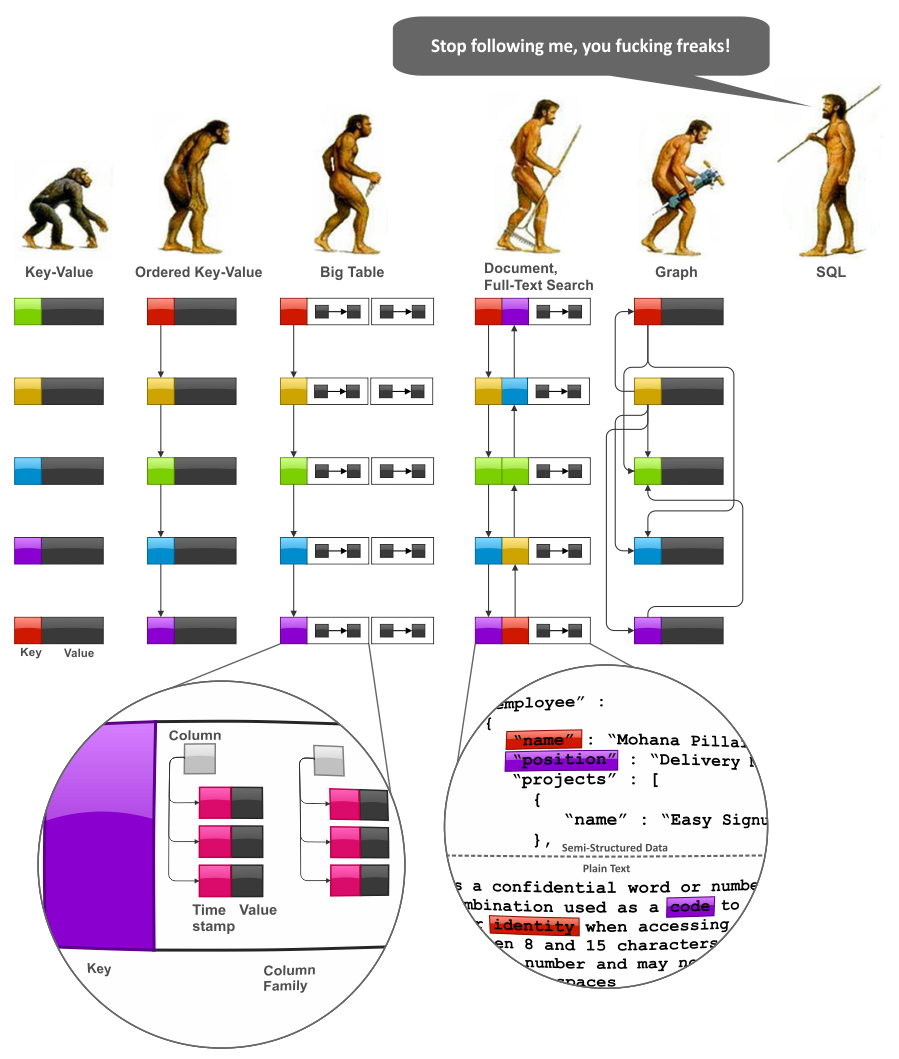
\includegraphics[width=\textwidth]{images/databases-overview.png}
    \caption{Übersicht Klassen an Datenbanken}
    \label{fig:klassen-datenbanken}
\end{figure}
